\section{The Role of the Corticospinal Tract}

It must have felt uncanny to those early researchers to find that surface stimulation of the cortex produces discrete muscle responses, in a way so similar to what Galvani did with the frog's leg. Indeed, Sherrington himself conveys the feeling clearly in the opening of his seminal lecture on the motor cortex \cite[p.271]{Sherrington1906}, confessing ``that although it is not surprising that such territorial subdivision of function should exist in the cerebral cortex, it is surprising that by our relatively imperfect artifices for stimulation we should be able to obtain clear evidence thereof.''

Of course, it did not go unnoticed that this fact might be due to the massive projection from cortex to the spinal cord, which had been fully traced by Türck only twenty years before Fritsch and Hitzig's experiment \cite{Nathan1955}. This so-called ``pyramidal'' tract\footnote{The name ``pyramidal'' is derived from the fact that the tract passes through the medullary pyramids, a pair of white matter structures in the brainstem with a roughly pyramidal shape.} was found to originate in the anterior regions of the cerebral cortex and terminate directly in the lateral columns of the spinal cord after decussating (i.e. crossing over) at the level of the brainstem's \emph{medulla oblongata}. The presence of this corticospinal tract presented compelling visual evidence of the means by which the motor cortex might be able to exert such a direct influence on movement by electrical conduction of nerve impulses, but the underlying biological mechanism remained elusive.

\subsection{A Functional Theory for the Motor Cortex}

Only four years after the discovery of the motor cortex, the Ukrainian anatomist and histologist Vladimir Betz connected for the first time the macroscopic cerebral organization and function proposed by Hitzig and Ferrier with unique, detailed histological evidence of cells found in the motor region, in his remarkably insightful 1874 publication:

\blockquote[{\protect\cite{Betz1874, Kushchayev2012}}]{Such consistency in the region where these cells can be found, manifested as a very definitive cortical layer, as well as in a specific cerebral convolution, prompted me to devote my attention to that particular part of the animal brain, mainly the dog’s, in which Fritsch and Hitzig achieved such brilliant physiological results, i.e. the lobe which borders the cruciate sulcus. I now found such cells of the same shape and in exactly the same position in nests in the dog, precisely in the lobe just mentioned. So in the dog, as well as in man, they are imbedded in the fourth cortical layer and occur only in this lobe and in the anterior half of the posterior (postcentral) convolution bordering it. In the dog, they are somewhat smaller, but nevertheless are the largest in its entire nervous system. They also possess two large and many small processes, and the inner process runs into a genuine nerve filament. In the area where they are found there are also many axis cylinders visible in the white substance, which run in the same direction as in the human. Undoubtedly these cells have all the attributes of the so-called ‘motor cells’ and very definitely continue as cerebral nerve fibres.}

Furthermore, in the same article he distinguishes between sensory and motor poles in the brain, placing the division in the central sulcus: ``The sulcus of Rolando divides the cerebral surface into two parts; an \emph{anterior} in which the large pyramidal nerve cells predominate, and a \emph{posterior}---including the temporal lobes---in which the cell layers are the same'' \cite{Betz1874,Clarke1996}.

In this way, Betz founded the hypothesis that these cells, which he called ‘giant pyramids’ were the cells of origin of the corticospinal tract, and that it were their impulses propagating down to the spinal cord that initiated the muscle responses evoked by electrical stimulation of the cortical surface. His early assignment of these giant cells to cortical layer four was essentially correct, although his layer four would today be considered layer five due to refinement of the total number of layers in cortical tissue \cite{Kushchayev2012}.

When the landmark works of Campbell and Brodmann elucidated in detail the cytoarchitectural features of the mammalian cortex, they both included extensive treatments of the pre-central ‘motor’ region and its unique anatomical arrangement \cite{Campbell1905,Brodmann1909}. In regard to the cells of Betz, Campbell in particular provided great clarification on their pattern of distribution and possible physiological function. After extensive histological examination of cortical tissue in the brains of the anthropoid ape and normal human subject, as well as examination of pathological material from cases of Amyotrophic Lateral Sclerosis and from patients that underwent amputation of a body part, he proposed in his monograph a histological basis for assigning the influence of different areas of the pre-central region to different muscle groups, suggesting that ``the largest (motor) cells are exactly those whose impulses have to travel down to the muscles of the lower extremity, those for the arm being quite a third smaller'' \cite[p.33]{Campbell1905}. He argued on the basis of similarity in anatomical configuration and retrograde degeneration studies that most likely even smaller pyramidal cells can form part of the corticospinal tract, becoming one of the first to suggest that a classification of Betz cells based purely on size was probably erroneous.

In addition to the characterization of the ‘motor’ cortex by its prominent layer V containing giant pyramidal cells, both Campbell and Brodmann noted clearly that the pre-central region showed a dramatic reduction in granular layer IV\footnote{For this reason, the frontal ‘motor’ cortices are also sometimes referred to as \emph{agranular} cortex.}. In the canonical layered arrangement of cortical tissue, layer IV is a dense layer of cell bodies known as the granular layer that separates superficial from deep layers. Functionally, layer IV is described as the target of feed-forward projections from sensory thalamus, making it the first layer of the cortex to receive direct sensory input. The observation that this layer was dramatically reduced in the pre-central motor region provided further suggestive evidence that the frontal cortices were more concerned with ‘output’ than with ‘input’.

\begin{figure}
\begin{center}
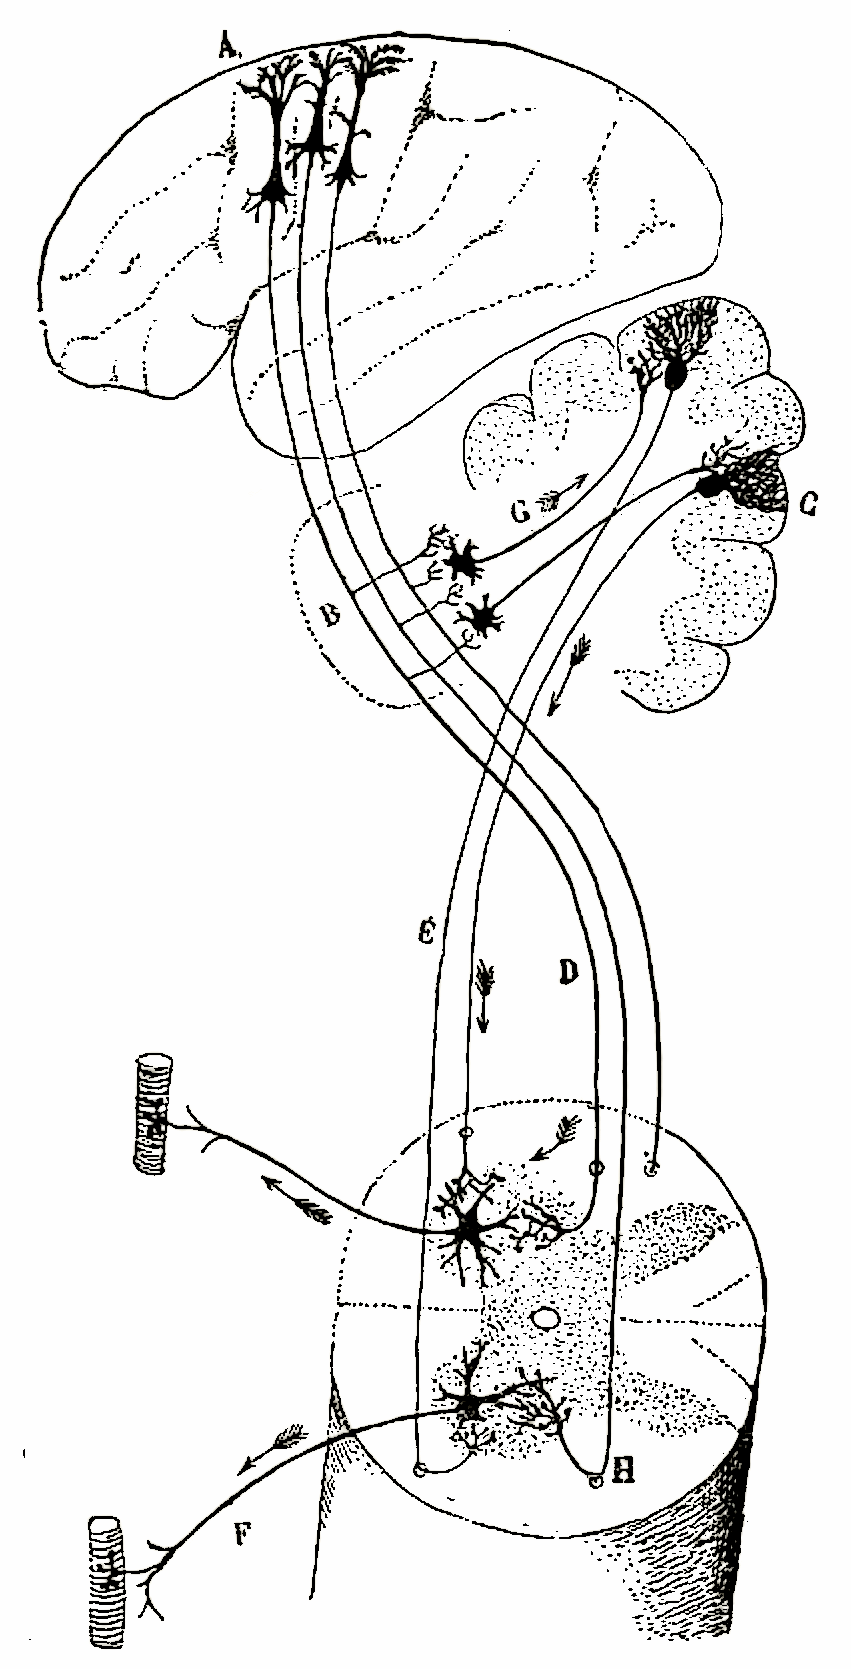
\includegraphics[width=0.65\columnwidth]{chapters/figuresChTeleology/cajalPathway}
\end{center}
\vspace{-5mm}
\caption{Schematic of the direction of impulses in the tactile sensory pathway and the voluntary movements pathway. A, pyramidal pathway; B, motor cells; C, D, sensory cells; E, cuneate nucleus of Burdach; F, gracile nucleus of Goll; G, central sensory pathway. The arrows indicate the direction of impulses \protect\cite[p.540]{RamonYCajal1909}.}
\label{fig:cajalPathway}
\end{figure}

The last remaining question was to explain how surface stimulation of the cortex was so effective if the subcortically projecting cells were located in the deep layers. This last piece of the puzzle was finally resolved with the development of the Golgi stain and the characterization of the full structure of the cortical pyramidal cell presented in Ramon y Cajal's anatomical masterpiece \cite{RamonYCajal1894,RamonYCajal1909}. In his work, he describes in detail the descending circuit for voluntary movements (Figure \ref{fig:cajalPathway}): ‘centrifugal’ excitation originates in the tufts of the long apical dendrites which extend vertically from the soma of deep pyramidal cells all the way into the superficial layers, and then descends to the spinal cord through the axons of the corticospinal pathway, crossing at the medullary pyramids \cite{RamonYCajal1909}. In the same figure he describes the symmetric tactile sensory pathway, flowing in the opposite direction from spinal cord to the somatosensory cortices \cite{RamonYCajal1909}, completing the sketch of the circuit which transported neural impulses from sensory stimulation to the perception and reasoning centres, and from there to muscle activation.

\subsection{The Effects of Lesions in the Corticospinal Tract}

In the wake of the Goltz-Ferrier debates, investigations of the role of the direct corticospinal descending pathway were conducted in multiple animal species. Sherrington himself started out his work by tracing spinal cord degeneration over large periods of time (up to 11 months) following cortical lesions in Goltz's dogs \cite{Langley1884,Sherrington1885}. He confirmed that many of the properties of the corticospinal tract in the primate held for the dog, and furthermore became one of the first to observe the presence of a degenerated ``re-crossed'' pyramidal tract that travels down the cord ipsilateral to the side of the lesion \cite{Sherrington1885}. These fibers would later come to be called the ipsilateral, ventral corticospinal tract, and have since been found and described in most mammalian species as forming roughly 10\% of the entire corticospinal projections \cite{Kuypers1981,Brosamle2000,Lacroix2004}. However, he also had the chance during this time to observe first hand the negative effects of corticospinal degeneration following lesion, which had been previously reported by Goltz and others in a variety of non-primate specimens. In his own words:

\blockquote[{\protect\cite[p.189]{Sherrington1885}}]{That the pyramidal tracts are in the dog requisite for volitional~impulses to reach limbs and body seems negatived by the fact that the animal can run, leap, turn to either side, use neck and jaws, \&c. with ease and success after nearly, if not wholly, complete degeneration of these tracts on both sides. Further, after complete degeneration of one pyramid, there is in the dog no obvious difference between the movements of the right and left sides.}

Interestingly, he does note that \enquote{defect of motion is observable only as a clumsiness in execution of fine movements} \cite{Sherrington1885}. These observations once again stood out in stark contrast with lesion experiments reported by Ferrier in the monkey, where cauterization of specific motor cortical areas produced complete and persistent paralysis of the corresponding body parts \cite{Ferrier1884}. Years later, Sherrington would come back to the motor cortex with a new set of landmark studies on stimulation and ablation of the precentral region \cite{Grunbaum1903,GrahamBrown1913,Leyton1917}. In these studies together with Gr\"unbaum, Sherrington targeted motor cortical lesions to the excitable area of the arm or the leg and tracked the recovery of the animals over time. Following the initial paresis and loss of muscle control they observed dramatic recovery of most skilled motor acts, such as peeling open a banana or climbing cages \cite{Leyton1917}. In order to test whether the recovery process was due to cortical reorganization, they systematically stimulated the areas adjacent to the lesion as well as the motor cortex of the opposite hemisphere, but failed to evoke movements in the affected limb \cite{Leyton1917}, as would be expected if commands were traveling down the corticospinal tract in spared regions. Furthermore, subsequent ablation of those areas failed to produce any new impairments in the recovered limb, leaving Sherrington and his colleagues at a loss to find the locus of recovery \cite{Leyton1917}.

Glees and Cole would later introduce a set of more quantitative behavioural assays in the hope of tracking in detail the recovery of motor control \cite{Glees1950,Cole1952}. They studied the behaviour of monkeys solving various puzzle boxes following successive circumscribed lesions to the thumb, index and arm areas of the motor cortex. As Sherrington reported there was a quick recovery after an initial period of paralysis and loss of motor control. However, even though the monkeys fully recovered their ability to skillfully open the puzzle box, some subtle movement deficits and paresis in the control of fine movements of the digits was reported to persist \cite{Glees1950}. When stimulating motor cortical areas surrounding the circumscribed lesions, they were able to evoke movements in the impacted digits and reinstate the paretic symptoms after further ablation \cite{Glees1950}. This suggested the hypothesis that surrounding areas of the motor cortex could undergo reorganization following the lesion. However, an important difference to emphasize between these experiments and those of Sherrington is the fact that only relatively circumscribed motor cortical regions were removed in each surgery, whereas in the original Sherrington study the entire elbow, wrist, index, thumb and remaining digit motor areas were excised at once \cite{Leyton1917}, most likely causing degeneration of the entire corticospinal pathway for the affected limb. The presence of an intact corticospinal tract, excitability of movements to low-current stimulation and transient paretic symptoms following ablation thus seem to go hand in hand.

In the hopes of clarifying the confusion of which exact movements were controlled by cortex, other studies focused on lesions restricted to the corticospinal tract, using both unilateral and bilateral section at the level of the medullary pyramids \cite{Tower1940,Lawrence1968,Lawrence1968a}. The goal was to isolate the effects of all the individual descending pathways to the spinal cord and resolve once and for all the question of whether the corticospinal tract of the motor cortex was the source of all ``voluntary'' movements. Sarah Tower was the first to describe in detail the results of unilateral and bilateral pyramidotomy in primates, with and without lesion of the motor cortex \cite{Tower1940}. She summarized the condition as ``hypotonic paresis'', characterized by a loss of skeletal muscle tone and depression of the vasomotor system, along with general weakening of the reflexes involving the affected limb segments. Although all discrete usage of the hand and digits was eliminated, she did emphasize the clear presence of voluntary movements in the various purposeful compensations produced by the animals to deal with the affliction. Tower attributed these compensations to the preserved capacities of brainstem circuits.

A more definitive study to dissociate the effects of direct corticospinal and indirect brainstem descending pathways was conducted by Lawrence and Kuypers, and presented in their now classical publications \cite{Lawrence1968,Lawrence1968a}. Using the Kl\"uver board, a task where monkeys have to pick morsels of food from differently sized round holes, they observed that while normal monkeys routinely pick up the food by pinching individual bits with their fingers, monkeys with bilateral corticospinal lesions were mostly unable to perform this precise pincer movement, and instead employed coarser compensatory clasping strategies to retrieve the food \cite{Lawrence1968}. In addition, lesioned monkeys were consistently reported to be somewhat slower and less agile than normal animals. However, most of their overall movement repertoire was surprisingly preserved. Their final conclusions fit remarkably well with the initial observations of Sherrington in the dog, suggesting that the corticospinal pathways superimpose speed and agility on subcortical mechanisms, and provide the capacity for fractionation of movements such as independent finger movements \cite{Lawrence1968}. These observations recapitulate the effects of motor cortical lesions reported by Sherrington, but remain at odds with the primary stated role involving motor cortex, and the direct corticospinal tract, with the control of all voluntary movements.

\subsubsection*{There are anatomical differences in corticospinal projections between primates and other mammals}

In primates, the conspicuous effects of motor cortical lesion can also be induced by sectioning the corticospinal tract, the direct monosynaptic projection that connects motor cortex, and other cortical regions, to the spinal cord \cite{Tower1940,Lawrence1968}. In monkeys, and similarly in humans, this pathway has been found to directly terminate on spinal motor neurons responsible for the control of distal muscles \cite{Leyton1917,Bernhard1954} and is also thought to support the low-current movement responses evoked by electrical stimulation of the cortex, as evidenced by the increased difficulty in obtaining a stimulation response following section at the level of the medulla \cite{Woolsey1972}.

However, the corticospinal tract is by no means the only pathway from cortex to movement (Figure \ref{fig:descendingTaxa}). Motor cortex targets many other brain regions that can themselves generate movement. In fact, this specialized connection from telencephalon to spinal cord appeared only recently in vertebrate evolution \cite{TenDonkelaar2009}, and was further elaborated to include a direct connection from cortex to motor neurons only in some primate species and other highly manipulative mammals such as raccoons \cite{Heffner1983}. In all other mammals, including cats and rats, the termination pattern of the corticospinal tract largely avoids the motor neuron pools in ventral spinal cord and concentrates instead on intermediate zone interneurons and dorsal sensory neurons \cite{Kuypers1981,Yang2003}. Why then is there such a large dependency on this tract for human motor control? One possibility is that the rubrospinal tract---a descending pathway originating in the brainstem and terminating in the intermediate zone---is degenerated in humans compared to other primates and mammals \cite{Nathan1955,Nathan1982}, and is thought to play a role in compensating for the loss of the corticospinal tract in non-human species \cite{Lawrence1968a,Zaaimi2012}.

It thus seems likely that most mammals rely on ``indirect'' pathways to convey cortical motor commands to muscles. These differences in anatomy might explain the lack of conspicuous, lasting movement deficits following motor cortical lesion in non-primates, but leaves behind a significant question: what is the motor cortex actually controlling in all these other mammals?

\begin{figure}
\begin{center}
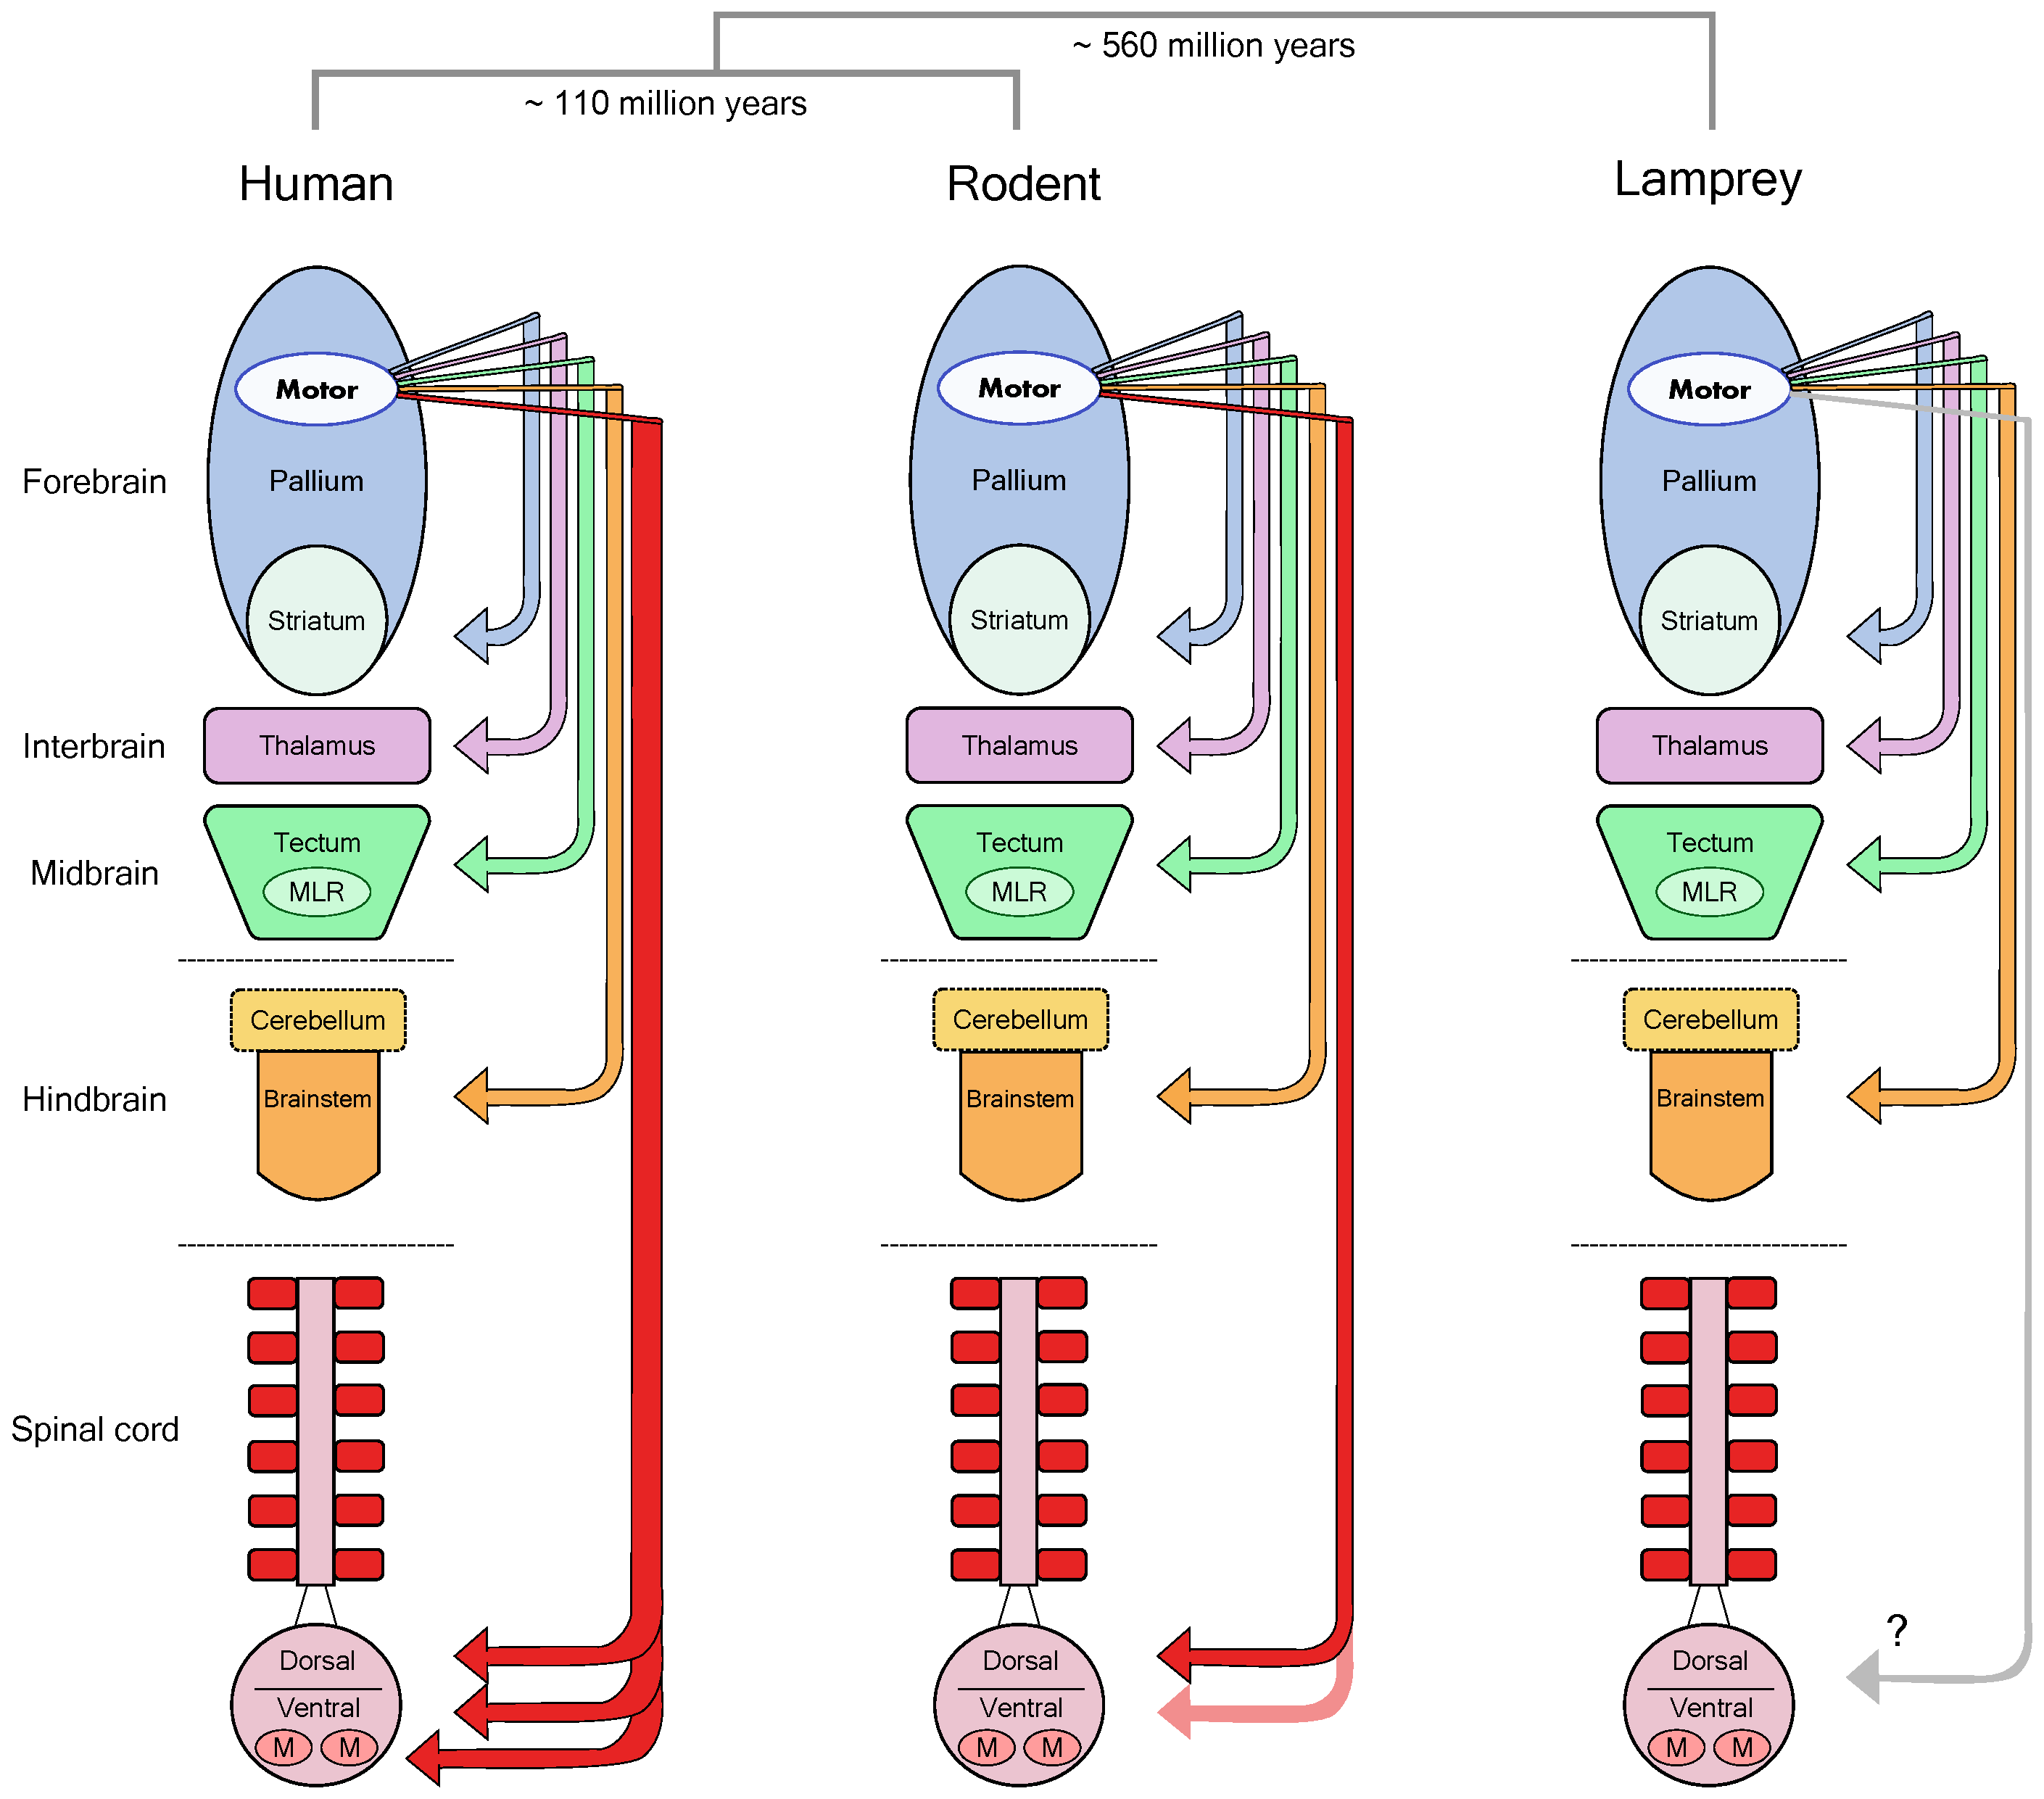
\includegraphics[width=\columnwidth]{chapters/figuresChTeleology/descendingTaxa}
\end{center}
\vspace{-5mm}
\caption{Forebrain motor control pathways across different vertebrate taxa. The molecular divergence times between human (primate), rodent and lamprey groups \protect\cite{Kumar1998} are noted above a schematic view of the major divisions in the vertebrate brain. Arrows indicate the descending monosynaptic projections identified in each group from motor regions of the forebrain pallium to lower motor centres. Note the specialized monosynaptic projection directly targeting spinal motor neurons in human. MLR, Mesencephalic Locomotor Region; M, Motor Neurons.}
\label{fig:descendingTaxa}
\end{figure}

\subsubsection*{What is the role of motor cortex in non-primate mammals?}

In the rat, a large portion of cortex is considered ``motor'' based on anatomical \cite{Donoghue1982}, stimulation \cite{Donoghue1982,Neafsey1986} and electrophysiological evidence \cite{Hyland1998}. However, the most consistently observed long-term motor control deficit following motor cortical lesion has been an impairment in supination of the wrist and individuation of digits during grasping, which in turn impairs reaching for food pellets through a narrow vertical slit \cite{Whishaw1991,Alaverdashvili2008a}. Despite the fact that activity in rodent motor cortex has been correlated with movements in every part of the body (not just distal limbs) \cite{Hill2011,Erlich2011}, it would appear we are led to conclude that this large high-level motor structure, with dense efferent projections to motor areas in the spinal cord \cite{Kuypers1981}, basal ganglia \cite{Turner2000,Wu2009}, thalamus \cite{Lee2008}, cerebellum \cite{Baker2001} and brainstem \cite{Jarratt1999}, as well as to most primary sensory areas \cite{Petreanu2012,Schneider2014}, evolved simply to facilitate more precise wrist rotations and grasping gestures. Maybe we are missing something. Might there be other problems in movement control that motor cortex is solving, but that we may be overlooking with our current assays?

